\part{Capitulo 3}
\vspace{-0.3cm}

\begin{center}
    \begin{large}
        Elementos de Meteorología
    \end{large}
\end{center}

La meteorología es la ciencia que estudia los fenómenos ocurridos en la atmósfera (vientos, presipitaciones, etc). Puede estar enfocada en el clima a largo o corto plazo.

\begin{itemize}
    \item Clima (largo plazo): Promedio de las condiciones que se mantienen en un periodo años y esta definido por medias de tendencia central (media, mediana, etc) o variabilidad (rango, desviación estándar, etc).
    \item Tiempo (corto plazo): Conjunto de características físicas que se dan en un tiempo y lugar determinado.
\end{itemize}

\section{Atmósfera}
La atmósfera cumple 3 funciones fundamentales:

\begin{enumerate}
    \item Almacenamiento de los vapores de agua de los procesos de evaporación y evotranspiración.
    \item Almacenamiento de calor y absorción de la radiación solar
    \item Medio de transporte para el vapor de agua, el cual se precipita.
\end{enumerate}

\subsection{Composición}

\begin{figure}[H]
    \centering
    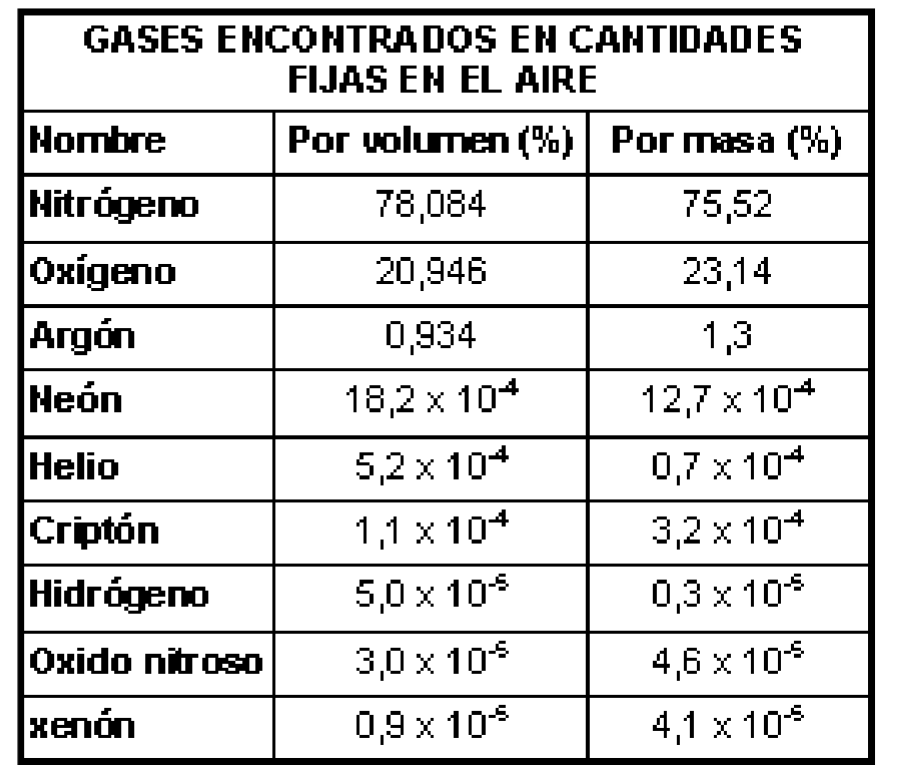
\includegraphics[width=0.5\textwidth]{imagenes/atm.png}
    \label{fig:composicion_atmosfera}
    \\
    \textbf{Contenido de vapor de agua varía entre 1-5\%}
\end{figure}

\subsection{Gases de efecto invernadero (GEI)}

\begin{itemize}
    \item Vapor de agua
    \item Dioxido de Carbono $CO_2$
    \item Metano $CH_4$
    \item Oxido Nitroso $N_2O$
    \item Ozono $O_3$
\end{itemize}

\subsection{Capas de la atmósfera}

\begin{enumerate}
    \item Troposfera: 0-13 km, contiene mayor parte del vapor de agua y es donde se desarrollan los fenómenos meteorológicos. Temperatura desciende hasta los -60°C.
    \item Estratosfera: 13-25 km, contiene la capa de ozono y temperatura constante a -60°C.
    \item Mesosfera: 25-80 km.
    \item Ionósfera: Absorbe las radiaciones de onda corta e ioniza moléculas.
    \item Exosfera: 500-1000 km, donde se encuentran los satélites. Se desvance gradualmente.
\end{enumerate}

\subsection{Circulación atmosférica}

Movimiento a gran escala de las masas de aire en la atm ocasionado por procesos térmicos y la rotación de la tierra.
\\\\
La energía que transmite el Sol a la Tierra no es homogénea. En los polos se reciben aprox. 90 $W/m^2$, mientras que en el ecuador se reciben 270 $W/m^2$. Esta diferencia provoca la transferencia de calor desde el ecuador a los polos, mediante celdas de convección y advección. Dado los continentes, mares y rotación, la transferencia de calor se realiza en 3 celdas:
\begin{itemize}
    \item Tropical
    \item Central
    \item Polar
\end{itemize}

\subsubsection{Celda de circulación vertical (Celda de Hadley)}

Como consecuencia de la diferencia de la distribución de energía en la tierra (radiación), el aire en el ecuador se calienta mucho más que el de los polos. 
\\\\
Si se supone tierra homogénea y en reposo, en el ecuador el aire al calentarse se eleva, a capas más altas, siendo sustituido por aire frio procedentes de los polos, ocurriendo una doble circulación de aire.

\begin{itemize}
    \item Del ecuador hacia los polos en las capas altas
    \item De los polos hacia el ecuador en las capas bajas
\end{itemize}

Esto no ocurre porque las masas de aire caliente al elevarse sufren un enfriamiento radiativo, provocando un aumento en su densidad y obligandolas a descender y calentarse adiabáticamente, conllevando una divergencia de dos subcorrientes superficiales, hacia el ecuador y hacia los polos.
\\\\
Esto define una celda cerrada en los trópicos (Celda de Hadley), con vientos del este hacia el ecuador (alisios) y vientos del oeste en altura a los polos (contraalisios).
\\\\
El aire que se mueve hacia los polos en el hemisferio sur adquiere un movimiento hacia el oeste, lo que ayuda a mantener la rotación de la Tierra. Cuando este aire llega a latitudes de 55°-60°, se encuentra con aire frío y seco que viene de los polos, formando el frente polar.
\\\\
El aire que converge hacia el frente polar asciende, creando dos nuevas celdas: una con corrientes hacia los polos (celda Polar) y otra con corrientes hacia el ecuador (celda Central).
\\\\
En realidad, la circulación general de la atmósfera se altera por la distribución de océanos y continentes, variaciones del relieve, vientos locales y sistemas de presión asociados a ciclones o anticiclones. Esto define los climas: secos en los polos y latitudes de 30º, y lluviosos en los trópicos.
\\\\
En Chile:

\begin{itemize}
    \item Zona Norte: Permanentemente bajo altas presiones. Desértica y bajas pps. 
    \item Zona Central: Mixto, húmeda en invierno y seca en verano
    \item Zona sur: Determianda por el frente polar. LLuvia siempre
    \item Zona polar: Alta presión, fría y seca. 
\end{itemize}

Las corrientes de mar dependen de los continentes y definen patrones de temperatura. Tienen efecto en el clima de una región.
En Chile, la corrinte de Humbolt es fría de S-N, modera las temperaturas.

\subsection{Presión atmosférica}

La presión atmosférica es el peso del aire sobre la superficie. Las curvas que representan igual presión se llaman isobaras, y su uso en cartas isobáricas permite caracterizar y predecir el clima.

\[
1 \, \text{atm} = 1 \, \text{bar} = 1.033 \, \text{kg/cm}^2 = 1013 \, \text{hPa} = 760 \, \text{mm Hg} = 14.7 \, \text{lb/in}^2
\]

\begin{equation}
    log(P_{atm}) = 2,882 - H/19500
\end{equation}

Donde $P_{atm}$ es la presión atmosférica (mm Hg) y H es la altitud (msnm)

\subsubsection{Centro de alta presión (Anticiclones)}

Proporcionan estabilidad atmosférica y constituyen barreras meteorológicas de desplazamiento de frentes, perturbaciones y tormentas.

\subsubsection{Centro de baja presión (Ciclones)}

Dan inestabilidades y perturbaciones atmosféricas que condicionan y suelen dar origen a precipitaciones y tormentas.

\section{Vientos}

Producen transferencias de calor y vapor de agua que condicionan fenómenos del ciclo hidrológico (Evaporación, evapotranspiración, derretimiento de nieves y hielos, formación de precipitaciones y desplazamiento de tormentas).
\\\\
Se originan por gradientes barométricos, en el sentido decreciente de dicho gradiente.
\\\\
Tipos de vientos:
\begin{itemize}
    \item Globales
    \item Regionales o locales
\end{itemize}

Los vientos de miden con un Anenómetro y la dirección se clasifica según su proveniencia
\\\\
Distribución del viento: dentro de la capa límite atmosférica

\begin{equation}
    \frac{v_1}{v_2} = \left(\frac{z_1}{z_2}\right)^p \quad \text{,} \quad p \approx \left[\frac{1}{7}, \frac{1}{3}\right]
\end{equation}

Si la atmósfera es neutra: Ley de von Kármán-Prandtl

\section{Radiación Solar}

\begin{itemize}
    \item Principal fuente energética para el desarrollo de los procesos físicos en la Tierra.
    \item La distribución estacional de esta energía depende de las características orbitales de la Tierra alrededor del Sol.
    \item Se propaga a la velocidad de la luz.
\end{itemize}

\subsection{Ley de Stefan Boltzmann}

La emisión total de radiación viene dada por la ecuación: 

\begin{equation}
    Re = e \times \sigma \times T^4
\end{equation}

Donde:
\begin{itemize}
    \item $e = $ emisividad de la superficie. ($e = 1$, cuerpo negro y $e = 0.97$, superficie del agua)
    \item $\sigma = 5.68 \times 10^{-8} (W/m^2 * K^4)$
    \item T = temperatura superficie en K  
\end{itemize}

\subsection{Ley de Wien}
La longitud de onda es inversamente proporcional a la temperatura de la superficie.

\begin{equation}
    \lambda (m) = 2.90 \times 10^{-3} / T (K)
\end{equation}

\subsection{Radiación neta}

La intensidad de la radicación solar que llega a la parte superior de la atmosfera disminuye por los siguientes factores: dispersión en la atmosfera, absorción en las nubes y oblicuidad de la sup. de la tierra

Se mide con:
\begin{itemize}
    \item Piranómetro: mide radiación solar global
    \item Piroheliómetro: mide radiación solar directa
    \item Piroradiómetro: mide radiación total incidente 
    \item Radiómetro neto: mide balance de radiación 
\end{itemize}

\section{Temperatura del Aire}

La temperatura es una medida de la energía interna de un cuerpo asociada al movimiento de partículas.
\\\\
La distribución de temperatura en la superficie y en la atm es resultado del balance energético global.
\\\\
Disminuye con la latitud y la altitud.
\\\\
En zonas marinas hay poca variación de la temperatura, en zonas áridas la variación es muy grande

\begin{align}
    \text{Si } Rad_{solar} > Emision_{Tierra} &\Rightarrow T \text{ aumenta} \\
    \text{Si } Rad_{solar} < Emision_{Tierra} &\Rightarrow T \text{ disminuye}
\end{align}

La temperatura del aire se mide por convección:
\begin{itemize}
    \item A 1,5 m de altura
    \item A la sombra y con ventilación
    \item En caseras meteorológicas
    \item Se mide con termómetro de mercurio
\end{itemize}

\subsection{Estimación de la temperatura}

\begin{itemize}
    \item Temperatura media diaria:
    \begin{equation}
        \bar{T} = \frac{T_{max} + T_{min} + T_{08} + T_{16}}{4}
    \end{equation}
    \item En ausencia de datos intermedios:
    \begin{equation}
        \bar{T} = \frac{T_{max} + T_{min}}{2}
    \end{equation}
    \item En alturas grandes se usan globosondas
    \item Gradiente adiabático normal: Tropósfera
    \begin{equation}
        \frac{\partial T}{\partial z} \approx -6{,}5 \, \left[\text{C/km}\right]
    \end{equation}
\end{itemize}

La única capa de interés es la tropósfera. Bajo ciertas condiciones se puede producir una inversión térmica, es decir que aumenta la T° con la altura.
\begin{itemize}
    \item Efecto del ciclo diurno
    \item Presencia de campos de hielon o nieve
    \item Poco viento
    \item Aire seco
    \item Pocas nubes
\end{itemize}

\section{Masas de aire y frentes}

Una masa de aire es un volumen de aire con propiedades físicas y termodinámicas uniformes horizontalmente. Estas masas adquieren características como temperatura y humedad en sus regiones de origen, y se modifican al mezclarse con otras masas de aire. La superficie frontal es la zona de separación entre masas de aire con diferentes propiedades. En Chile, las masas de aire provienen principalmente del océano Pacífico y regiones subpolares.
\\\\
Los frentes cálidos se forman cuando una masa de aire caliente se desplaza y asciende sobre una masa de aire más frío, generando precipitaciones extensas, que pueden abarcar entre 100 y 300 km en la zona del aire frío.
\\\\
Los frentes fríos ocurren cuando una masa de aire frío avanza sobre una masa de aire más cálido, provocando el ascenso del aire caliente. Las precipitaciones resultantes son generalmente intensas y cubren áreas pequeñas, de 60 a 80 km, en la zona previamente ocupada por el aire caliente.
\\\\
Frente Ocluido: cuando un frente frío alcanza a un frente cálido, el aire frío se desplaza por debajo del aire cálido, formando un frente ocluido. Las precipitaciones son intensas y cubren áreas pequeñas.

\subsection{Estabilidad Atmosférica}

\begin{itemize}
    \item Gradiente termico normal: $\gamma = -6,5 \, \text{(°C/km)}$
    \item Gradiente adiabático seco: $\Gamma_d = 9,8 \, \text{(°C/km)}$ Gas ideal y seco
    \item Graduente pseudo adiabático y humedo: $\Gamma_s$
    \begin{figure}[H]
        \centering
        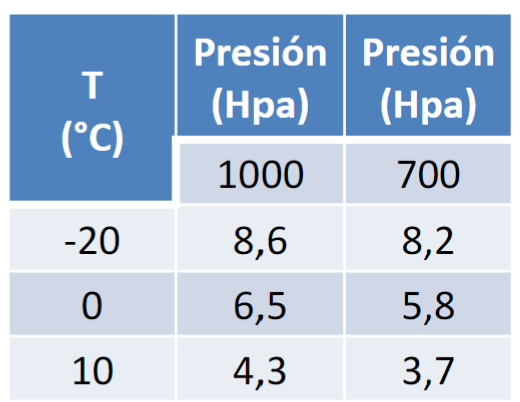
\includegraphics[width=0.3\textwidth]{imagenes/grad.png}
        \label{fig:gradiente}
    \end{figure}
\end{itemize}

La diferencia entre los gradientes tiene grandes implicancias en la estabilidad.
\\\\
Para que una masa de aire sea absolutamente estable, su gradiente de temperatura debe ser menor que el gradiente adiabático correspondiente: seco para aire seco y húmedo para aire saturado.

\begin{figure}[H]
    \centering
    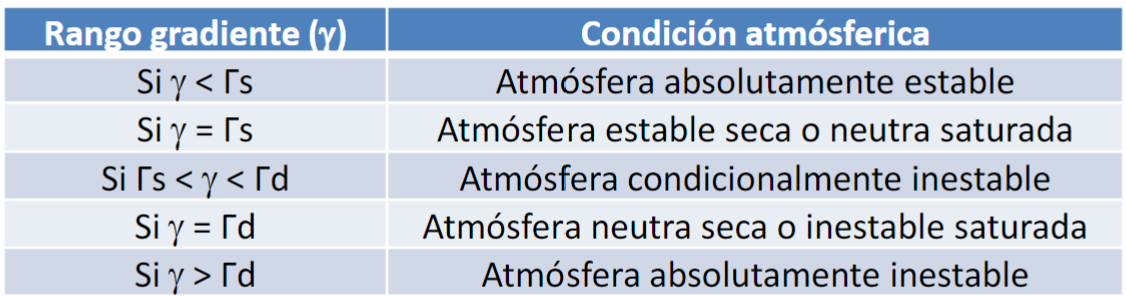
\includegraphics[width=0.5\textwidth]{imagenes/estabilidad.png}
    \label{fig:estabilidad}
\end{figure}

\section{Propiedades del vapor de agua}

Según la Ley de Dalton, la presión de vapor es la ejercida solo por el vapor de agua. La presión total de la atmósfera es la suma de la presión del aire seco y la del vapor de agua.

\begin{equation}
    e = \rho_v \cdot R_v \cdot T
\end{equation}

Donde:
\begin{itemize}
    \item $e = $ presión de vapor de agua (Pa)
    \item $\rho_v = $ densidad del vapor de agua (gr/m³)
    \item $R_v = $ constante de los gases para vapor de agua (J/kg K)
    \item $T = $ temperatura (K)
\end{itemize}

\begin{equation}
    P_{total} = P_{seco} + e
\end{equation}

\begin{equation}
    P_{seco} = \rho_d \cdot R_d \cdot T
\end{equation}

Donde: 
\begin{itemize}
    \item $\rho_d$ es la densidad del aire seco (gr/m³)
    \item $R_d$ es la constante de los gases para aire seco = 287 (J/kg K)
\end{itemize}

\begin{equation}
    P_{total} = \rho_d \cdot R_d \cdot T + \rho_v \cdot R_v \cdot T \quad ; \quad R_v = \frac{R_d}{0.622}
\end{equation}
    
\begin{equation}
    P_{total} = \rho_d \cdot R_d \cdot T + \rho_v \cdot \left(\frac{R_d}{0.622}\right) \cdot T
\end{equation}
    
\begin{equation}
    P_{total} = \left(\rho_d + \frac{\rho_v}{0.622}\right) \cdot R_d \cdot T
\end{equation}

Humedad específica: 
\begin{equation}
    q_v = 0,622 \cdot \frac{e}{P}
\end{equation}

\begin{equation}
    R_a = R_d \cdot \left(1 + 0.608 \cdot q_v \right)
\end{equation}

Para una temperatura del aire dada, el contenido máximo de humedad que el aire puede contener corresponde a la presión de vapor de saturación (\(e_s\)), que se puede calcular con una ecuación específica.

\begin{equation}
    e_s = 611 \cdot \exp\left(\frac{17.27 \cdot T}{237.3 + T}\right)
\end{equation}

Humedad relativa:
\begin{equation}
    R_h = \frac{e}{e_s}
\end{equation}

Temperatura de punto de rocío (\(T_d\)): es la temperatura a la que se debe enfriar una masa de aire húmedo para que se sature, manteniendo la misma presión y contenido de agua.
\\\\
Punto de rocío: temperatura a la que habría que enfriar el aire, manteniendo constante la presión de vapor, para que se sature. En este punto se cumple:

\begin{equation}
    e = e_s \cdot T_R
\end{equation}

\section{Humedad Atmosférica}








